% !TEX TS-program = pdflatex
% !TEX encoding = UTF-8 Unicode

% This is a simple template for a LaTeX document using the "article" class.
% See "book", "report", "letter" for other types of document.

% \documentclass[10pt,twocolumn]{article} % use larger type; default would be 10pt
\documentclass[10pt]{article} % use larger type; default would be 10pt

\usepackage[utf8]{inputenc} % set input encoding (not needed with XeLaTeX)

%%% Examples of Article customizations
% These packages are optional, depending whether you want the features they provide.
% See the LaTeX Companion or other references for full information.

%%% PAGE DIMENSIONS
\usepackage{geometry} % to change the page dimensions
\geometry{a4paper} % or letterpaper (US) or a5paper or....
\geometry{margin=1.2in} % for example, change the margins to 2 inches all round
% \geometry{landscape} % set up the page for landscape
%   read geometry.pdf for detailed page layout information

\usepackage{graphicx} % support the \includegraphics command and options

% \usepackage[parfill]{parskip} % Activate to begin paragraphs with an empty line rather than an indent

%%% PACKAGES
\usepackage{booktabs} % for much better looking tables
\usepackage{array} % for better arrays (eg matrices) in maths
\usepackage{paralist} % very flexible & customisable lists (eg. enumerate/itemize, etc.)
\usepackage{verbatim} % adds environment for commenting out blocks of text & for better verbatim
\usepackage{subfig} % make it possible to include more than one captioned figure/table in a single float
% These packages are all incorporated in the memoir class to one degree or another...

%%% HEADERS & FOOTERS
\usepackage{fancyhdr} % This should be set AFTER setting up the page geometry
\pagestyle{fancy} % options: empty , plain , fancy
\renewcommand{\headrulewidth}{0pt} % customise the layout...
\lhead{}\chead{}\rhead{}
\lfoot{}\cfoot{\thepage}\rfoot{}

%%% SECTION TITLE APPEARANCE
\usepackage{sectsty}
\allsectionsfont{\sffamily\mdseries\upshape} % (See the fntguide.pdf for font help)
% (This matches ConTeXt defaults)

%%% ToC (table of contents) APPEARANCE
\usepackage[nottoc,notlof,notlot]{tocbibind} % Put the bibliography in the ToC
\usepackage[titles,subfigure]{tocloft} % Alter the style of the Table of Contents
\renewcommand{\cftsecfont}{\rmfamily\mdseries\upshape}
\renewcommand{\cftsecpagefont}{\rmfamily\mdseries\upshape} % No bold!

%%% My Own Packages
\usepackage{tcolorbox}  % for pretty bounding boxes

%%% END Article customizations

%%% The "real" document content comes below...

\title{COMP4107 Project Report}
\author{Christian Abbott TODO number}
\date{Basim Ramadhan 100 901 646} % Activate to display a given date or no date (if empty),
% otherwise the current date is printed 

\begin{document}
	\maketitle
	
	\section{Running Our Program}
	
	TODO create a readme
	
	
	
	\begin{tcolorbox}
		\begin{verbatim}
		make prepare-venv
		source env/bin/activate
		python train.py & 
		python evaluate.py &
		tensorboard --logdir=$(pwd)/logs
		\end{verbatim}
	\end{tcolorbox}
	
	The commands above will perform the following:
	
	\begin{enumerate}
		\item Create a virtual environment with the required libraries.
		\item Enter the virtual environment.
		\item Initialize a new classifier and start training it.
		\item Repeatedly evaluate the classifier's accuracy so far.
		\item Start TensorBoard to monitor the classifier's accuracy.
	\end{enumerate}
	
	\section{The Problem Being Solved}
	
	For our project we investigated and compared the performance of the state-of-the-art in CNN's for image recognition with the ImageNet dataset. We decided to use the Tiny ImageNet\footnote{https://tiny-imagenet.herokuapp.com/} dataset for our project because the entire ImageNet dataset proved to be too computationally expensive for us when we tried using it in the beginning. This reduced dataset contains 200 classes to recognize, as opposed to the 1000 classes in full ImageNet. We wanted to learn about different researchers efforts in tackling the ImageNet dataset. We wanted to create our own classifier for recognizing images from the Tiny ImageNet dataset based on what those researchers did. The classifier models we implemented and compared are "reduced" versions of the originals. In other words, we tried to compress them and retain classification accuracy.
	
	\subsection{Experimental Methodology}
	
	\subsection{Baseline CNN Architecture}
	
	For our experiments, we implemented classifier models based on the works of different researchers. In the beginning, we implemented a very simple CNN on our own. This simple model will provide a baseline to compare other models to.
	
	\subsection{SimpleNet}
	
	For our experiments, we implemented classifier models based on the works of different researchers. In the beginning, we implemented a very simple CNN on our own. This simple model will provide a baseline to compare other models to.
	
	\subsection{VGG 16}
	
	For our experiments, we implemented classifier models based on the works of different researchers. In the beginning, we implemented a very simple CNN on our own. This simple model will provide a baseline to compare other models to.
	
	\subsection{AlexNet}
	
	For our experiments, we implemented classifier models based on the works of different researchers. In the beginning, we implemented a very simple CNN on our own. This simple model will provide a baseline to compare other models to.
	
	\section{Our Best Classifier}
	
	\begin{tcolorbox}
		\textbf{Architecture:}
		\begin{itemize}
			\setlength\itemsep{-0.3em}
			\item Convolution 3x3
			\item Max Pooling 2x2
			\item Fully connected 1024
			\item Fully connected 200
		\end{itemize}
	\end{tcolorbox}
	
	\subsection{Hyperparameters}
	
	\begin{itemize}
		\item[\textbf{Learning Rate}] $0.00TODO$
	\end{itemize}
	
	\section{Limitations}
	
	1. Limited GPU power.
	
	2. Limited time means we couldn't work out all the issues.
	
	\section{Conclusion \& Future Work}
	
	The end!
	
	\section{References}
	\begin{itemize}
		\item https://arxiv.org/abs/1608.06037 \\ (SimpleNet)
		\item https://arxiv.org/abs/1409.1556 \\ (VGG 16)
		\item https://papers.nips.cc/paper/4824-imagenet-classification-with-deep-convolutional-neural-networks.pdf \\ (AlexNet)
		\item https://arxiv.org/abs/1412.6071 \\ (Fractional Pooling)
		\item http://scott.fortmann-roe.com/docs/BiasVariance.html
		\item TODO
		\item TODO
		\item TODO
	\end{itemize}
	
	\section{Figures}
	
	\subsection{Baseline CNN Architecture \& Results}
	\begin{tcolorbox}
		\textbf{Architecture:}
		\\ TODO add RELU to all architecture boxes
		\begin{itemize}
			\setlength\itemsep{-0.3em}
			\item Convolution: 3x3
			\item Max Pooling: 2x2
			\item Fully connected: 1024
			\item Fully connected: 200
			\item Softmax
		\end{itemize}
	\end{tcolorbox}
	
	
	\subsection{SimpleNet Architecture \& Results}
	\begin{tcolorbox}
		\textbf{Architecture:}
		\\ TODO I used simplenetC
		\begin{itemize}
			\setlength\itemsep{-0.3em}
			\item Convolution: 2x2
			\item Convolution: 2x2
			\item Convolution: 1x1
			\item Convolution: 2x2
			\item Max Pooling: 2x2
			\item Convolution: 2x2
			\item Convolution: 2x2
			\item Max Pooling: 2x2
			\item Convolution: 2x2
			\item Max Pooling: 2x2
			\item Convolution: 2x2
			\item Convolution: 2x2
			\item Max Pooling: 2x2
			\item Convolution: 2x2
			\item Convolution: 1x1
			\item Convolution: 1x1
			\item Max Pooling: 2x2
			\item Convolution: 2x2
			\item Max Pooling: 2x2
			\item Convolution: 1x1
			\item Softmax
		\end{itemize}
	\end{tcolorbox}
	
	\subsection{VGG16 Architecture \& Results}
	\begin{tcolorbox}
		\textbf{Architecture:}
		\begin{itemize}
			\setlength\itemsep{-0.3em}
			\item Convolution: 2x2
			\item Convolution: 2x1
			\item Convolution: 1x2
			\item Max Pooling: 2x2
			\item Convolution: 2x2
			\item Convolution: 2x2
			\item Convolution: 2x2
			\item Max Pooling: 2x2
			\item Convolution: 2x2
			\item Convolution: 2x1
			\item Convolution: 1x2
			\item Max Pooling: 2x2
			\item Fully Connected: 200
			\item Softmax
		\end{itemize}
	\end{tcolorbox}
	
	\subsection{AlexNet Architecture \& Results}
	\begin{tcolorbox}
		TODO I'm using XL
		\textbf{Architecture:}
		\begin{itemize}
			\setlength\itemsep{-0.3em}
			\item Convolution: 11x11, stride 4
			\item Convolution: 5x5
			\item Max Pooling: 3x3, stride 2
			\item Convolution: 3x3
			\item Convolution: 3x3
			\item Convolution: 3x3
			\item Max Pooling: 3x3
			\item Convolution: 3x3
			\item Convolution: 3x3
			\item Convolution: 3x3
			\item Max Pooling: 3x3
			\item Fully Connected: 4096
			\item Fully Connected: 4096
			\item Fully Connected: 200
			\item Softmax
		\end{itemize}
	\end{tcolorbox}
	
	\subsection{Computational Graph}
	We used TensorBoard to visualize our final model. Unfortunately, the graph wasn't as neatly organized as we would have liked. We hope the following snippets from the computational graph are useful:
	\begin{figure}[htbp,width=0.5em]
		\centering
		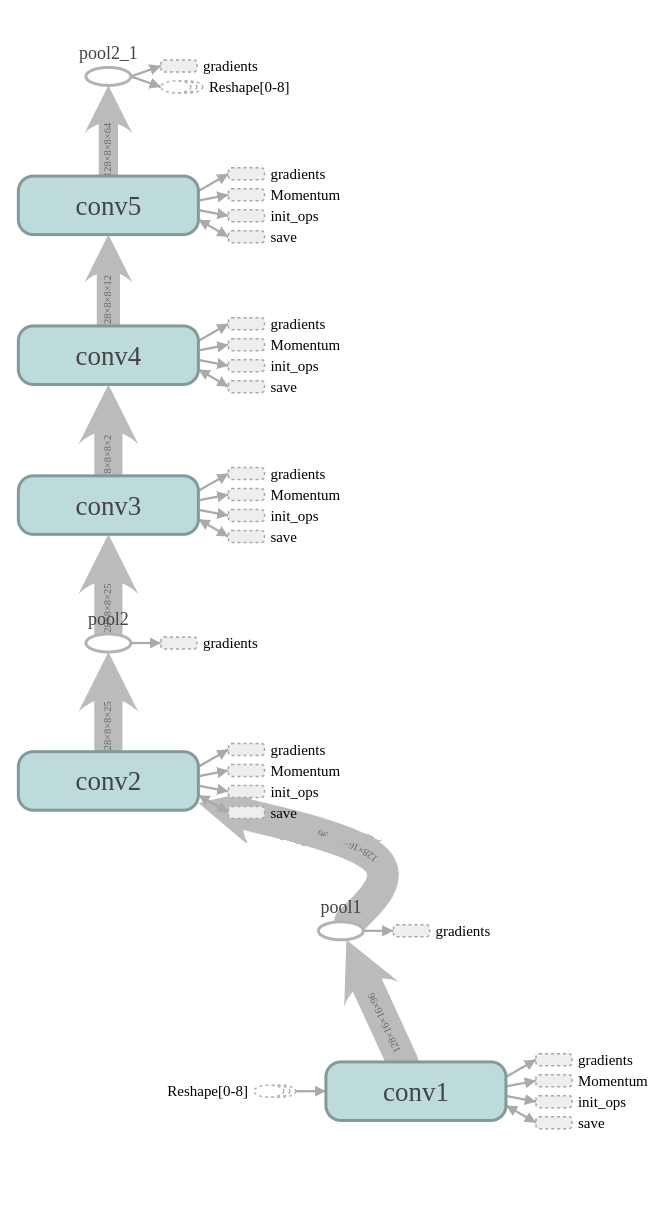
\includegraphics{./figures/graph-1.png}
		\caption{accuracy.png}
	\end{figure}
	
	
\end{document}
